% !TeX root = ../thuthesis-example.tex

\chapter{模型建立与应用}

\section{使用药材配对直接分析处方效果的尝试}

在引入更复杂的模型前,一个自然的想法是探究参与构成有效处方和不参与的药材配对在基因关联强度上是否有显著差异。如果这种假设成立,我们便可以直接通过评价药方中药材配对的好坏来分析其有效性。

\subsection{基于基因关联图连通部分减少数的分析}

我们可以沿用之前分析处方“二冬膏”时使用图的连通度的方法,批量地考察药材配对后是否能够显著减少基因关联图的连通部分数。如果出现这种情况,说明这两种药材联合使用可能共同作用于某些生物通路,起到互补的作用。可以对处方药材配对和随机药材配对作出如下的分布图进行对比:

\begin{figure}[H]
  \centering
  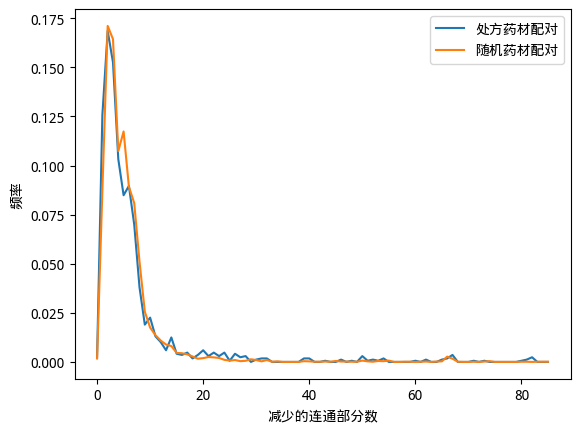
\includegraphics[width=\linewidth]{component_reduction_pdf.png}
  \caption{处方和随机药材配对减少的基因关联图连通部分数分布}
  \label{fig:component_reduction_pdf}
\end{figure}

\begin{figure}[H]
  \centering
  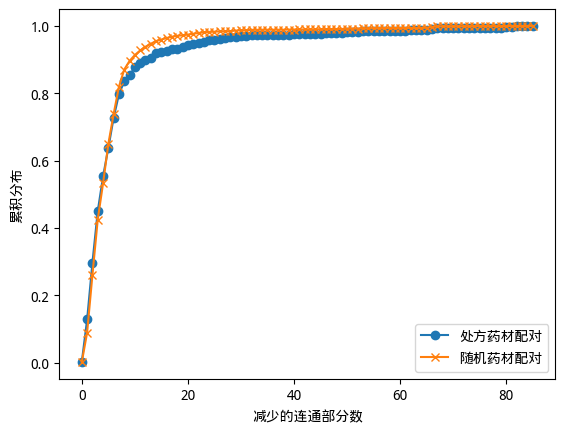
\includegraphics[width=\linewidth]{component_reduction_cdf.png}
  \caption{处方和随机药材配对减少的基因关联图连通部分数累积分布}
  \label{fig:component_reduction_cdf}
\end{figure}

此时双样本Kolmogorov-Smirnov检验的$D$值为$0.0409$,$p$值为$0.015$,可以得到显著差异,说明处方中已有的药材配对倾向于更多地减少基因关联图中的连通部分,这可能是药材配对的有效性的一个重要特征。

\subsection{基于网络分数增益的分析}


为了应用定量信息,我们可以考察药材配对之间增加的关联边数或者边权重之和,然后将真实的药材配对和所有可能药材配对分别进行排序,作出增益-分位数曲线,从而比较“是否属于已知处方”能否带来统计差异。同时,我们也可以尝试使用基因在药材中通过化合物的定量信息,观察增加这个额外信息相比仅使用STRING给出的分数是否能给出更显著的统计差异。下图是在应用与不应用化合物定量信息的条件下作出的对比曲线:

\begin{figure}[H]
  \centering
  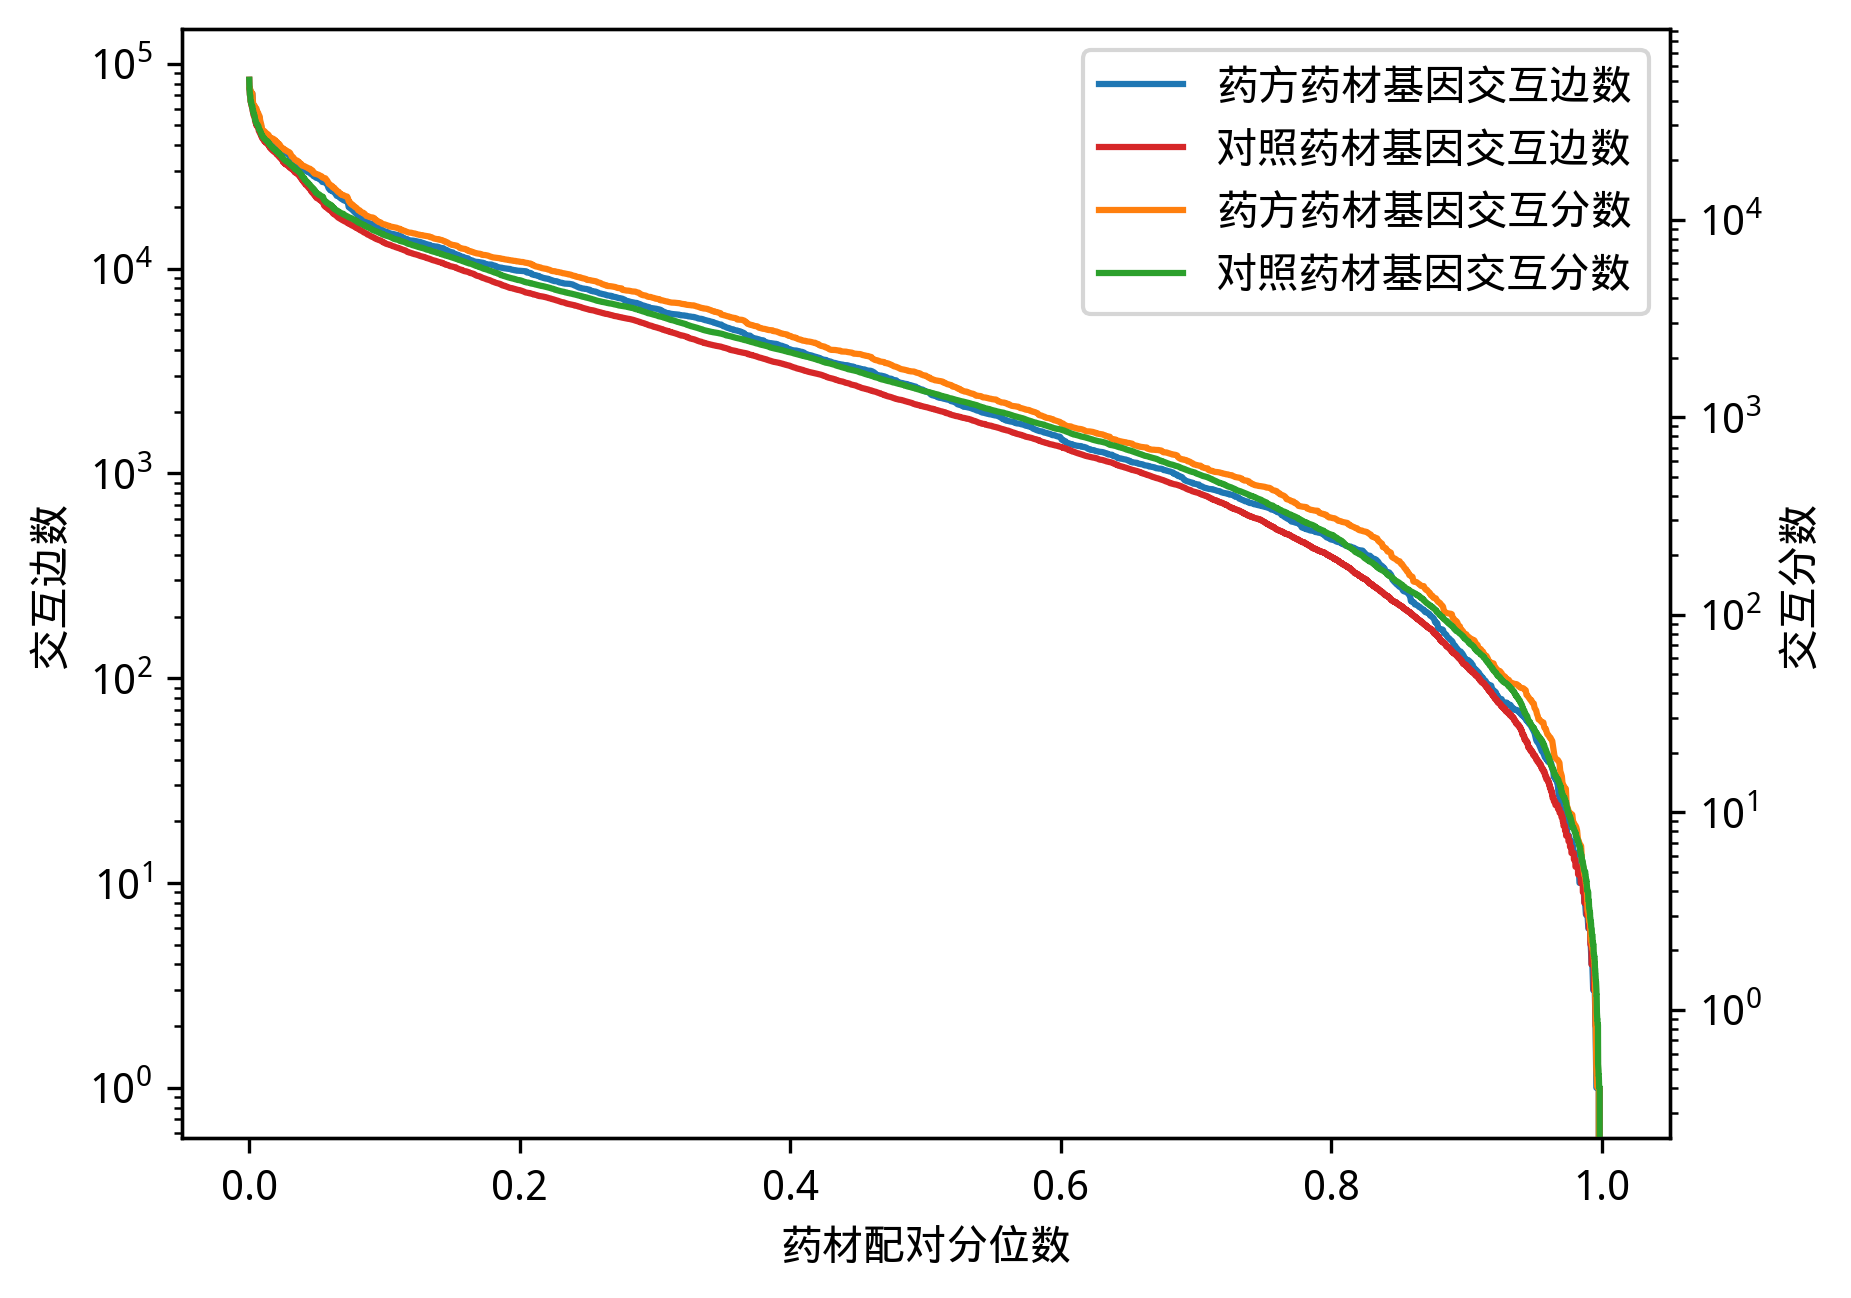
\includegraphics[width=0.95\linewidth]{scores_without_weight.png}
  \caption{不使用化合物定量的药材配对边数/分数增益-分位数曲线}
  \label{fig:score_without_weight}
\end{figure}

\begin{figure}[H]
  \centering
  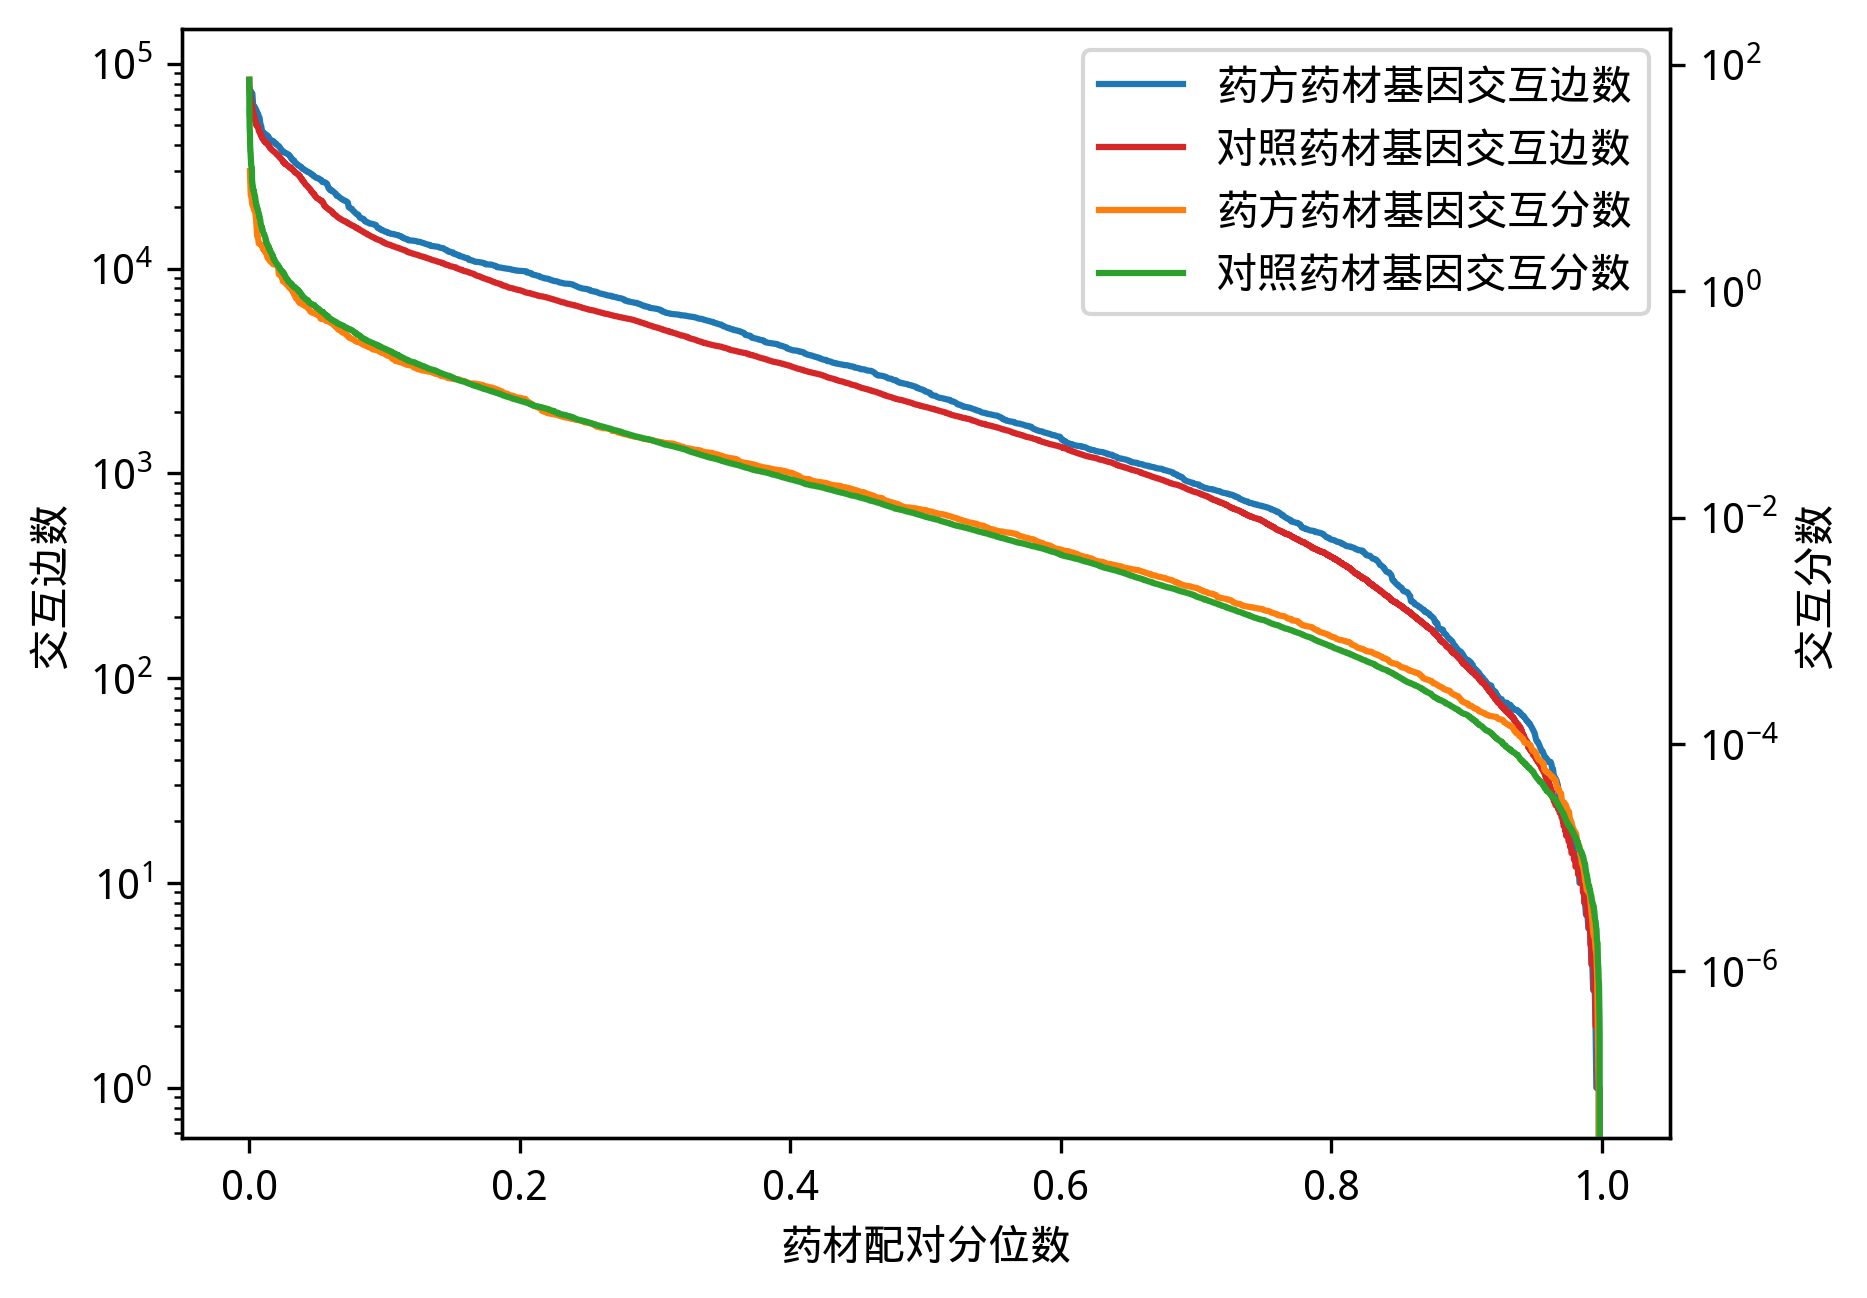
\includegraphics[width=0.95\linewidth]{scores_with_weight.png}
  \caption{使用化合物定量的药材配对边数/分数增益-分位数曲线}
  \label{fig:scores_with_weight}
\end{figure}


虽然我们无法简单地通过边数或分数增益准确地判断药材配对的有效性,但是我们可以从图线中直观地看到,如果不应用化合物定量信息,属于已知处方的药材配对在边数和分数上,几乎各个分位数点处都有优势。使用双样本Kolmogorov-Smirnov检验,可以得到边数的$D$值为$0.0551$,$p$值为$0.00029$,分数的$D$值为$0.05556$,$p$值为$0.00024$,即这两种指标均能说明是否属于已知药方会导致显著差异,而引入STRING关联分数可以略微提升置信度。

然而,当我们在此引入化合物含量信息后,从图线上发现,增益曲线的差异性几乎消失,甚至有明显的反转区域;双样本Kolmogorov-Smirnov检验的$D$值为$0.0243$,$p$值为$0.35$,无法得到显著差异,这说明化合物含量信息的引入反而使得药材配对的边数和分数增益失去了区分性。这可能是因为化合物含量信息本身存在大量数量级层面的差异,直接相乘引入了过大的噪声。

为了解决上面的问题,我们考虑使用对化合物含量进行归一化,即使用 $\frac{(w_{a1}+w_{a2})(w_{b_1}+w_{b2})}{w_{a1}w_{b2}+w_{b1}w_{a2}}$来作为 1,2 两个药材中基因对 $(a, b)$ 的化合物定量权重。这样,我们可以得到如下的增益曲线:

\begin{figure}[H]
  \centering
  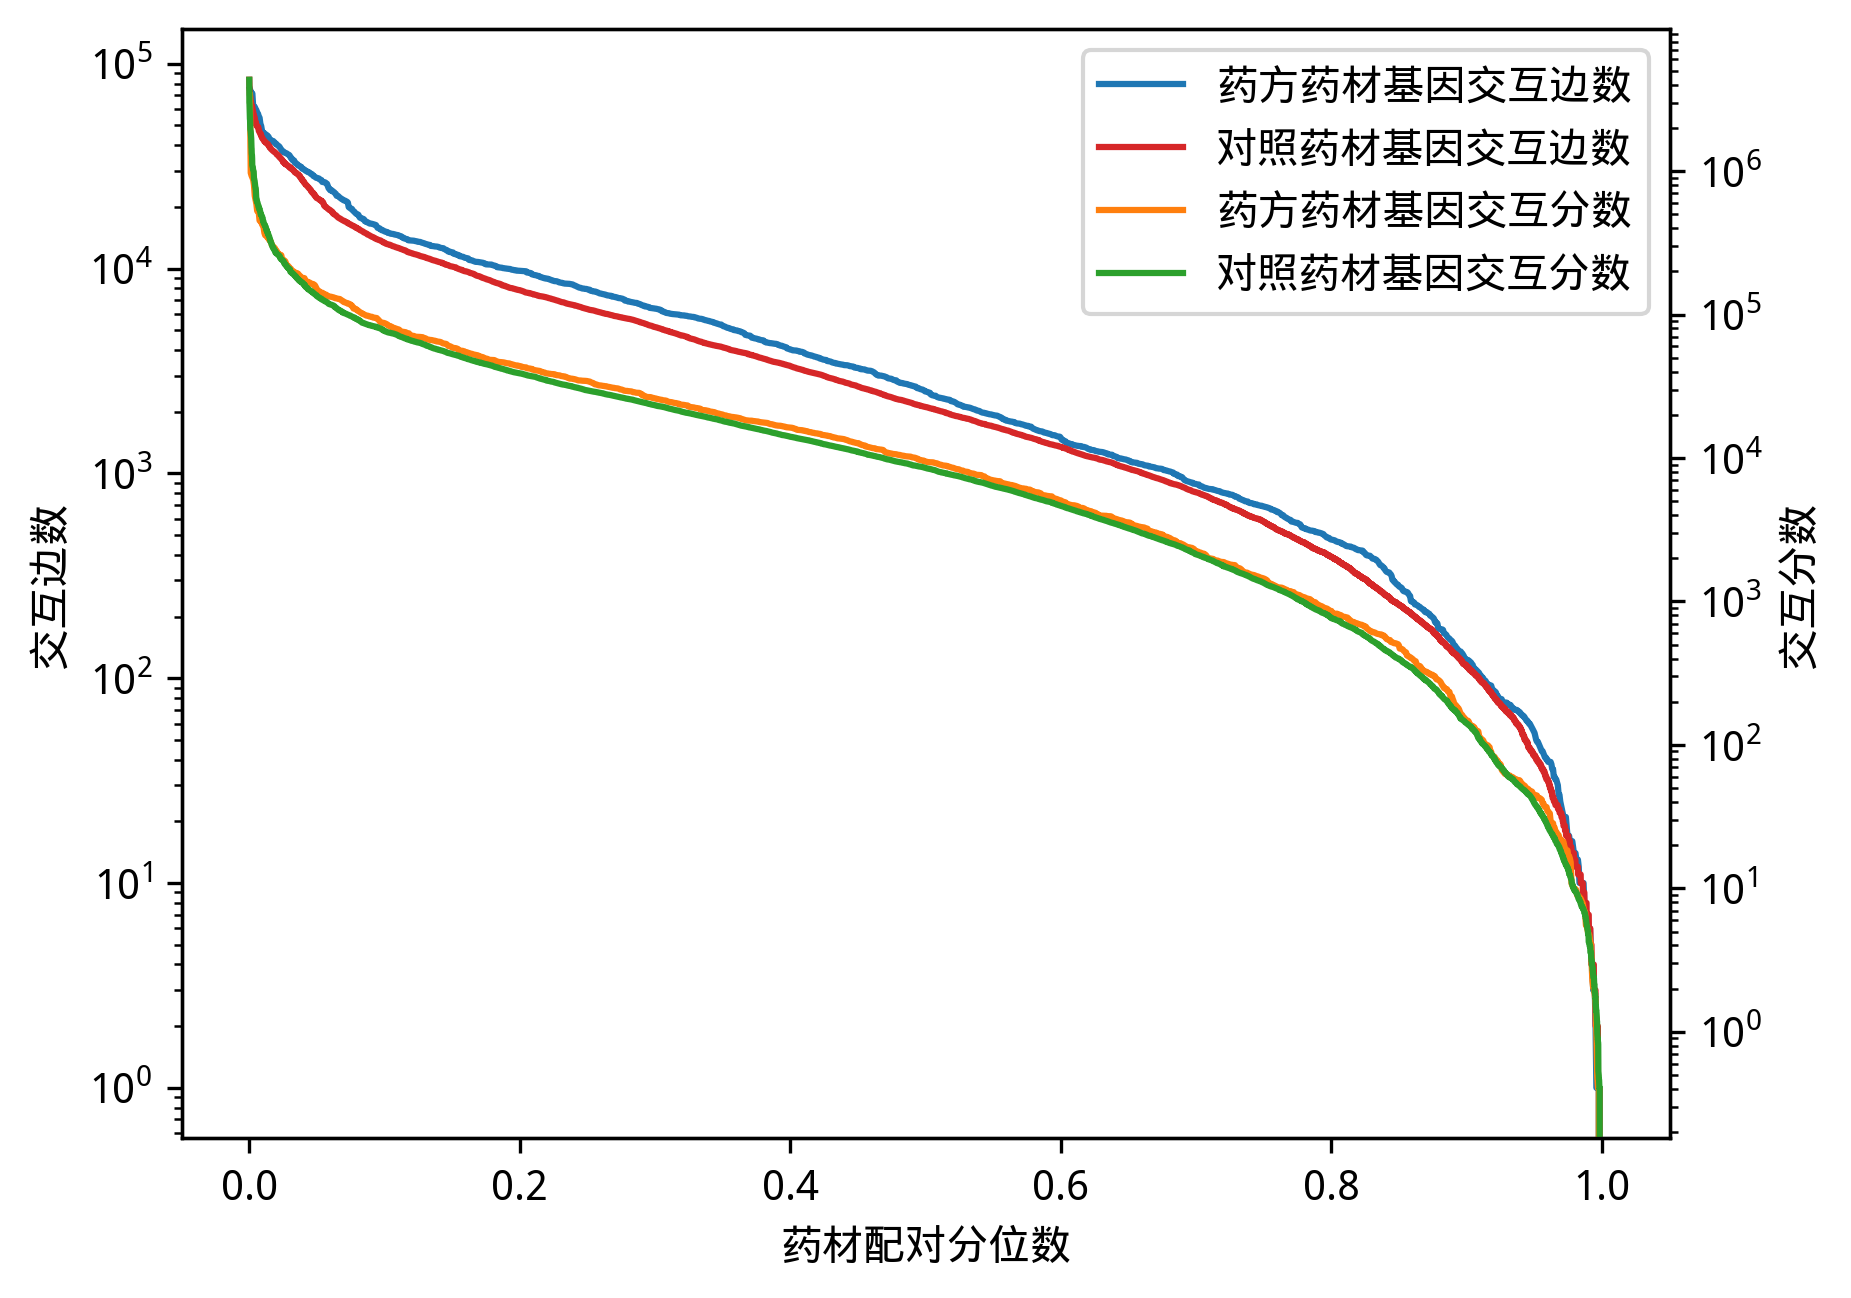
\includegraphics[width=0.95\linewidth]{scores_with_normalized_weight.png}
  \caption{使用归一化化合物定量的药材配对边数/分数增益-分位数曲线}
  \label{fig:scores_with_normalized_weight}
\end{figure}

这里的图线相比之前得到了改善,可以观察出药方药材配对几乎始终在对照药材配对上方,但双样本Kolmogorov-Smirnov检验具有$D$值为$0.0314$,$p$值为$0.11$,仍然没有显著性,说明对数在此问题中可能是一个更好的转换方式。但定量信息依然没有为药材配对的边数和分数增益带来提升,说明我们可能还需要建立更复杂的模型来运用定量信息解释处方的效果。

% edge
% KstestResult(statistic=0.05506882248177303, pvalue=0.0002908647549561178, statistic_location=5799, statistic_sign=-1)
% unweighted
% KstestResult(statistic=0.05564546832511763, pvalue=0.00024155665548500303, statistic_location=3674.2729999999983, statistic_sign=-1)
% weighted
% KstestResult(statistic=0.024379685069236018, pvalue=0.34918573567118794, statistic_location=0.0013520617904999987, statistic_sign=-1)
% normalized
% KstestResult(statistic=0.031446876287792414, pvalue=0.11124597693644322, statistic_location=13623.52746273345, statistic_sign=-1)

\section{使用图神经网络的处方效果预测}

如果从处方层面考虑问题,我们可以作出这样的假设:各基因受处方整体的作用等于处方中各药材影响的代数和,来自不同药材或不同化合物的基因影响在混同后是完全等价的。在这种假设下,我们可以直接遍历处方中的每个药材求和,得到每个基因的总表达影响,这样就把一个处方建模成了一系列以基因作为顶点,从化合物含量信息推出的总表达影响为点权重,基因之间的关联为边,STRING分数为边权重的图。利用图神经网络的方法,我们便可以训练模型对处方的效果进行预测,其中设《中国药典》中已经存在的处方为正例,而随机生成的、大概率不会有现实药理作用的处方为负例,便形成了一个通过图特征进行二分类的问题。这事实上是一个正无标签学习问题,我们没有确信的负例,即通过实验验证不存在任何正向药理作用的处方。这种情况下,由于正例是固定的,数量上非常有限,而负例可以通过从药材列表中任意选择,随机赋予定量,几乎无限地生成。相比于构造平衡的处方数据集,如果采样更多负例,即虚拟处方来训练,可能更有利于发现正例特有的特征。但是,这也会使得原有的准确率、召回率无法直接反映处方判别模型性能,需要使用采样、加权的方法克服这些问题。在本研究中,我们采用的是构建均衡样本的方法,但是模型实际调优时依然可以使用不均衡的策略。

在实际的训练和预测过程中,图的节点数,即处方中的药材数,会显著影响连接密度和图表示,是重要的特征,但有效处方的实际大小存在显著的区别,其中大小在8及以下的处方出现的频次较多。这一方面和指导处方配伍的中医传统理论有关,另一方面也可能是因为药材的定量信息不足,越大的处方越容易出现缺少药材定量而无法入选有效处方的情况。具体的分布如下:

% 此处存在较多留白,需要补充

\begin{figure}[H]
  \centering
  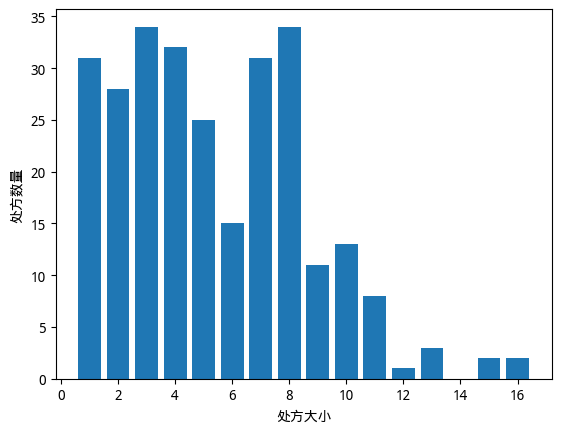
\includegraphics[width=\linewidth]{prescription_size.png}
  \caption{《中国药典》中药材均在ccTCM中收录的处方大小分布}
  \label{fig:prescription_size}
\end{figure}

为了防止学习到的实际上是有效处方较可能拥有的大小而非底层的关联信息,我们不能简单地随机指定生成虚拟药方的大小,而要使生成集合中各大小的处方比例也与《中国药典》中的已知处方相近。然而,从上述分布图中,我们可以看出处方大小9开始有一次显著的下降,而大小在12及以上的处方每个大小仅有0-3个已知记录。如果直接进行训练-验证-测试集的划分,将极有可能出现不均衡的现象,即较大而稀少的处方出现在训练和测试中的比例差别大,从而影响构造的类似大小负例的判别。因此,我们可以初步尝试直接去掉这些较大的处方,提高模型的稳定性,但更好的方法应是通过一定的采样策略来平衡数据集,比较建模效果,判断这些较大的处方样本是否含有标签推断中的重要信息。

另一方面,涉及药材非常少的较小处方也值得我们关注。这其中的一个特例是只含有一味药材的处方,即《中国药典》中分类的“单味制剂”,由于处方中药材的用量需要归一化,单味制剂药材权重始终为1,如果我们在随机构造中选取与现有单味制剂所用药材相同的药材,结果将与现有处方完全相同,将为正例而无标签例,在此这种情况出现的可能性显著高于规模更大的处方,因此需要特殊处理。除了这个较为显然的影响外,还有一种不容忽视的情况是较小的处方可能作为其他处方的子图存在。在这种情况下,一方面我们基于临床经验往往得以判定额外的药材至少不会对处方产生负面影响,即新的更大的处方应仍然是有效的;另一方面,这种有效性往往很难证明来自网络扩大后引入其他药材的影响,除非它们的实际生理药理作用有显著的不同,但这种不同在现有的,未结合临床征候的数据中没有得到体现。在这里,本研究的倾向是不考虑以有效子图为基础的扩大处方因此而获得的有效性,而关注其自身的特征,至少在模型学习的阶段不引入这个先验。这是因为建模的目标是发现构成有效药方的不同的基础特征,而不是单纯求取更好的预测性能。从临床实践的观点上看,这种策略有助于我们发现新的简单基础的有效药方,而不是扩大已有的处方,以数量取胜。

\subsection{基于图卷积网络的分析}

我们首先考虑了朴素的图卷积网络(GCN),它使用简单的层次化方法聚合节点的邻域信息,适合于这里的基因表达关联。应用GCN模型对处方是否真实存在的标签进行预测,实验环境的具体配置如下:


\begin{table}
  \centering
  \caption{实验环境配置}
  \begin{tabular}{ll}
    \toprule
    操作系统             & CentOS 7.5.1804                           \\
    CPU              & Intel(R) Xeon(R) Gold 6226R CPU @ 2.90GHz \\
    GPU              & Tesla V100-SXM2-32GB                      \\
    CUDA             & 11.4                                      \\
    cuDNN            & 7.5.1                                     \\
    Python           & 3.10.0                                    \\
    PyTorch          & 1.12.1                                    \\
    torch\_geometric & 2.5.3                                     \\
    scikit-learn     & 1.3.2                                     \\
    \bottomrule
  \end{tabular}
  \label{tab:three-line}
\end{table}

可在单卡上对此数据集进行常规规模的学习,得到的训练和测试曲线如下:

% 此处存在较多留白,需要补充

\begin{figure}[H]
  \centering
  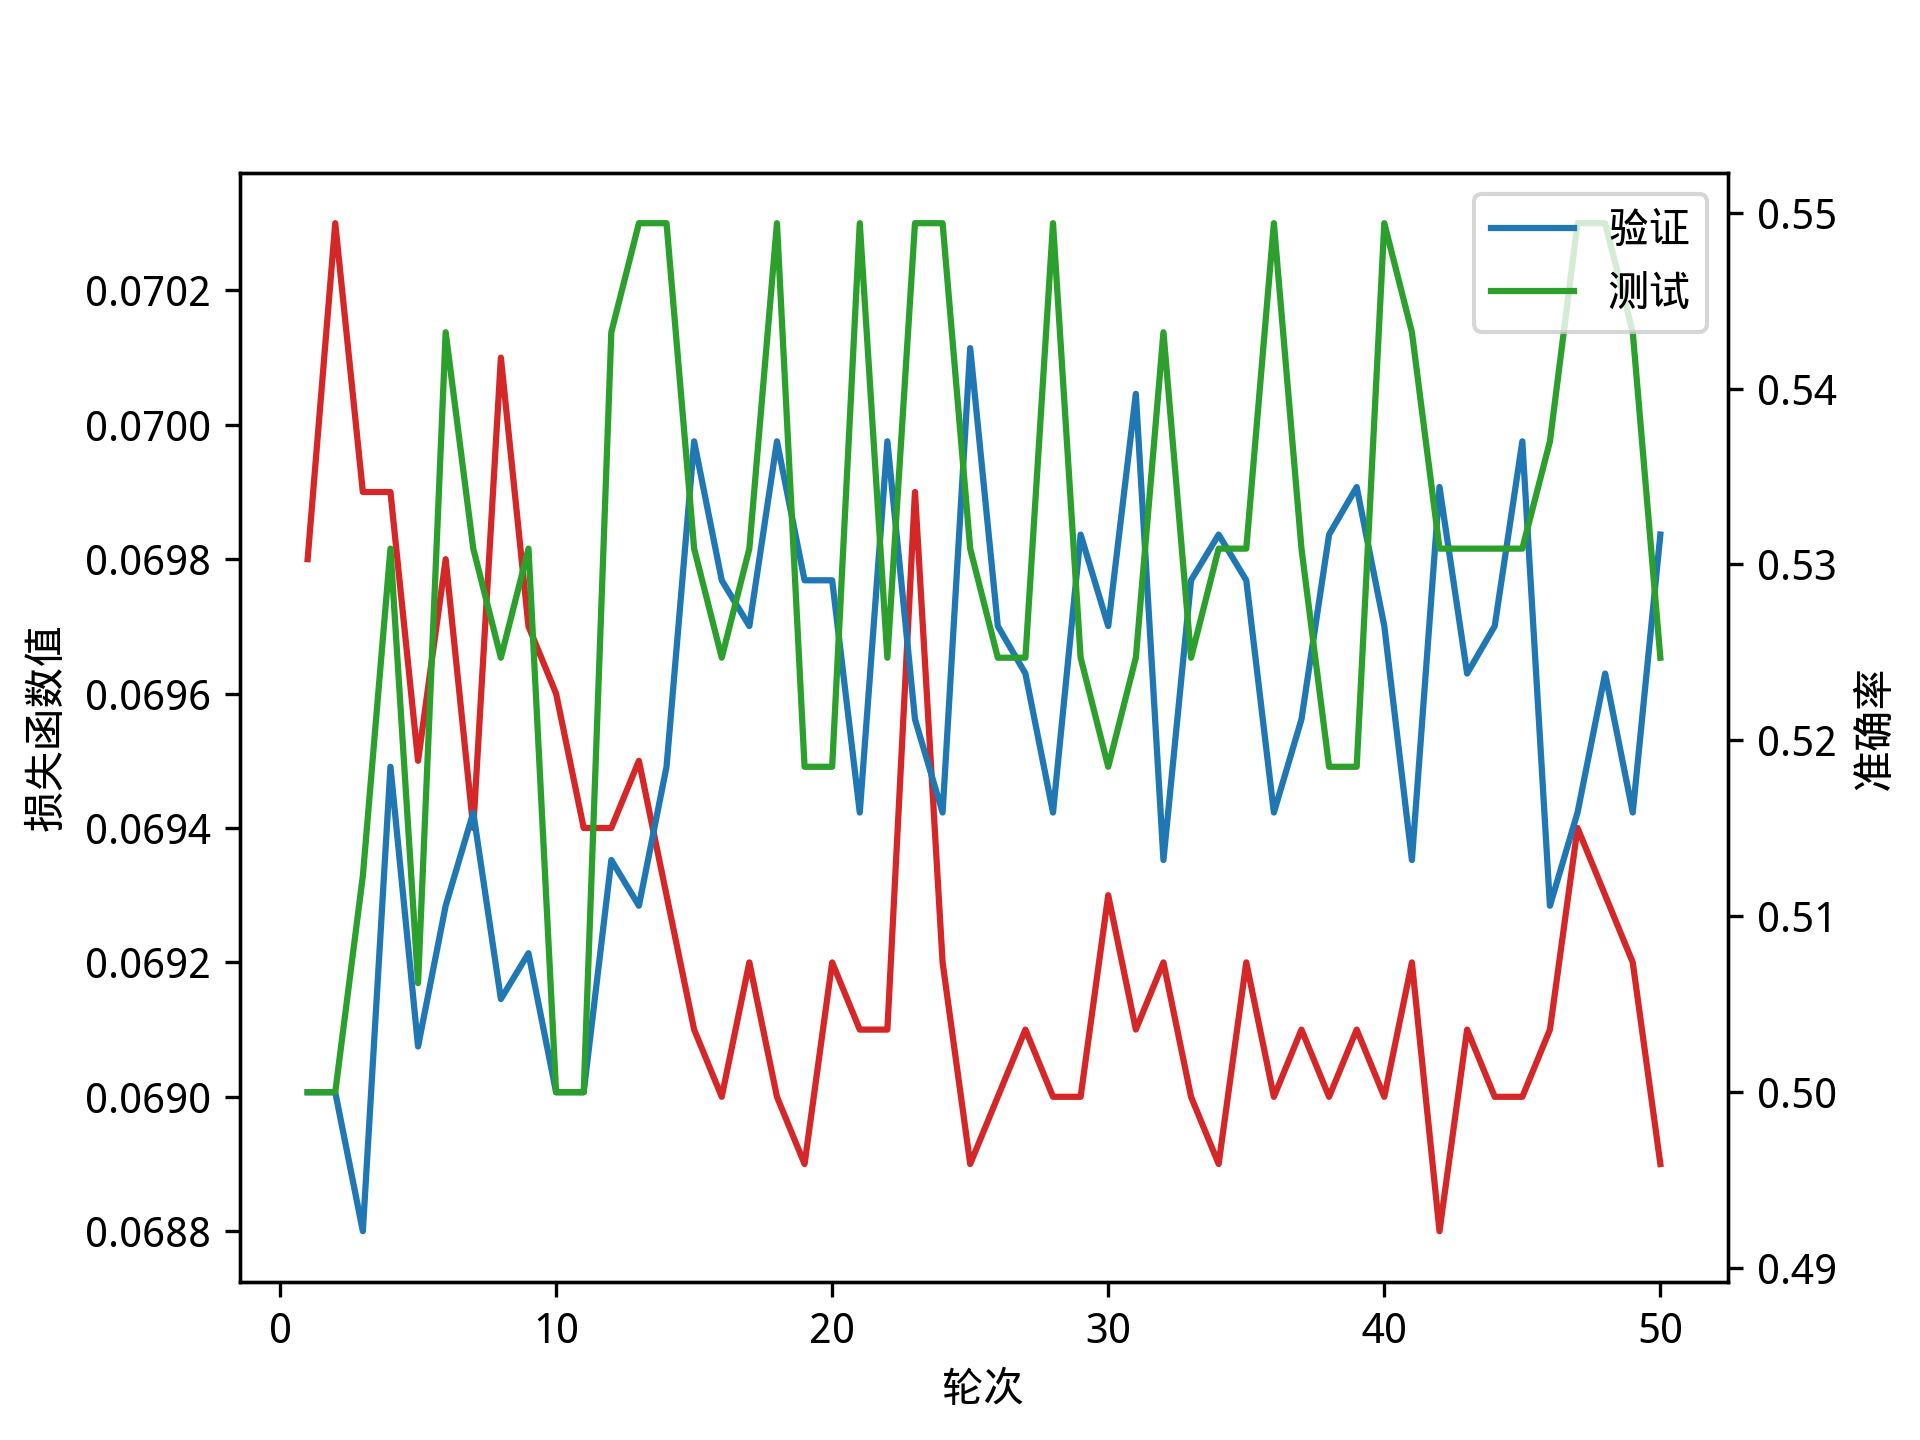
\includegraphics[width=\linewidth]{gcn_0.01.png}
  \caption{GCN模型的训练和测试曲线}
  \label{fig:gcn_train_curve}
\end{figure}

可能是由于化合物定量信息表征能力有限,或者没有选取更优的模型进行学习,得到的模型预测准确率的提升并不高,但至少稳定在0.5以上,均值达到0.53左右,至少说明了一定的预测能力。验证集和测试集上的处方标签预测正确率均处在比较低的水平上,大概率显示模型存在表征能力不足、欠拟合的问题。在这种情况下,我们可以考虑使用更适于表征学习的模型,如自编码器(autoencoder, AE)。

\subsection{基于自编码器的分析}

自编码器是一种主要为了将输入编码为压缩的、有意义的表示,然后重新解码,使得结果与最初输入尽可能接近,以学习无标签数据的抽象特征的神经网络,\cite{Bank_Koenigstein_Giryes_2021},最早由Rumelhart、Hinton和Williams等人在1986年提出\cite{10.5555/104279.104293}。在本研究中,我们首先定义了一个简单的图自动编码器,使用GCN层进行编码,全连接层进行解码,从而提取和重构处方的特征。在训练过程中,我们仅使用正例数据,直至逐元素的最小均方误差损失收敛。对于使用化合物含量信息作为节点权重的自编码器,在50个训练周期后收敛到 $3\times 10^{-5}$ 左右。


然后,我们提取图的低维表示。自编码器后可接不同的分类器,故我们选取了诸多经典的机器学习算法,包括逻辑回归、支持向量机、随机森林、梯度提升、AdaBoost、多层感知机、高斯朴素贝叶斯、K近邻,分别进行分类预测,并输出相应的分类报告,以进行分类器准确率、对处方正负例及加权平均意义下的精确率、召回率、F1分数等预测性能指标的比较。具体的实验结果如下:

\begin{table}[H]
  \centering
  \resizebox{\textwidth}{!}{%
    \begin{tabular}{lcccccccccc}
      \toprule
      \multirow{2}{*}{模型} & \multirow{2}{*}{准确率} & \multicolumn{3}{c}{正例} & \multicolumn{3}{c}{负例} & \multicolumn{3}{c}{加权平均}                                           \\
                          &                      & 精确率                    & 召回率                    & F1                       & 精确率  & 召回率  & F1   & 精确率  & 召回率  & F1   \\
      \midrule
      逻辑回归                & 0.537                & 0.52                   & 0.76                   & 0.62                     & 0.58 & 0.32 & 0.41 & 0.55 & 0.54 & 0.51 \\
      支持向量机               & 0.549                & 0.53                   & 0.90                   & 0.66                     & 0.68 & 0.21 & 0.32 & 0.60 & 0.55 & 0.49 \\
      随机森林                & 0.685                & 0.66                   & 0.76                   & 0.71                     & 0.72 & 0.61 & 0.66 & 0.69 & 0.69 & 0.68 \\
      梯度提升                & 0.654                & 0.62                   & 0.75                   & 0.68                     & 0.70 & 0.56 & 0.62 & 0.66 & 0.65 & 0.65 \\
      AdaBoost            & 0.537                & 0.53                   & 0.55                   & 0.54                     & 0.54 & 0.52 & 0.53 & 0.54 & 0.54 & 0.54 \\
      多层感知机               & 0.512                & 0.50                   & 0.70                   & 0.59                     & 0.53 & 0.33 & 0.41 & 0.52 & 0.51 & 0.50 \\
      朴素贝叶斯               & 0.519                & 0.51                   & 0.94                   & 0.66                     & 0.64 & 0.11 & 0.19 & 0.58 & 0.52 & 0.42 \\
      K近邻                 & 0.593                & 0.59                   & 0.60                   & 0.59                     & 0.60 & 0.59 & 0.59 & 0.59 & 0.59 & 0.59 \\
      \bottomrule
    \end{tabular}
  }
  \caption{应用化合物定量信息和基因关联的自编码器各分类器性能对比}
  \label{tab:performance_comparison}
\end{table}

可以看出,在参与比较的分类器中,随机森林取得了最高的准确率和加权平均F1分数,达到了0.685和0.69,显示出了较强的分类能力。使用这个模型,我们将可能区分一个新处方是否具有与成方相似的底层特征,从而对其有效性进行一定推断。为了判断化合物含量是否有助于提升模型预测准确率,我们在代码中进行相对应的修改,不再使用权重信息,即将每个关联边的点权重都设置为1。由于节点权重的数量级不同,在50个训练周期后,自编码器的损失函数收敛到 $0.06$ 左右。可以作出两组的训练曲线。

\begin{figure}[htbp]
  \centering
  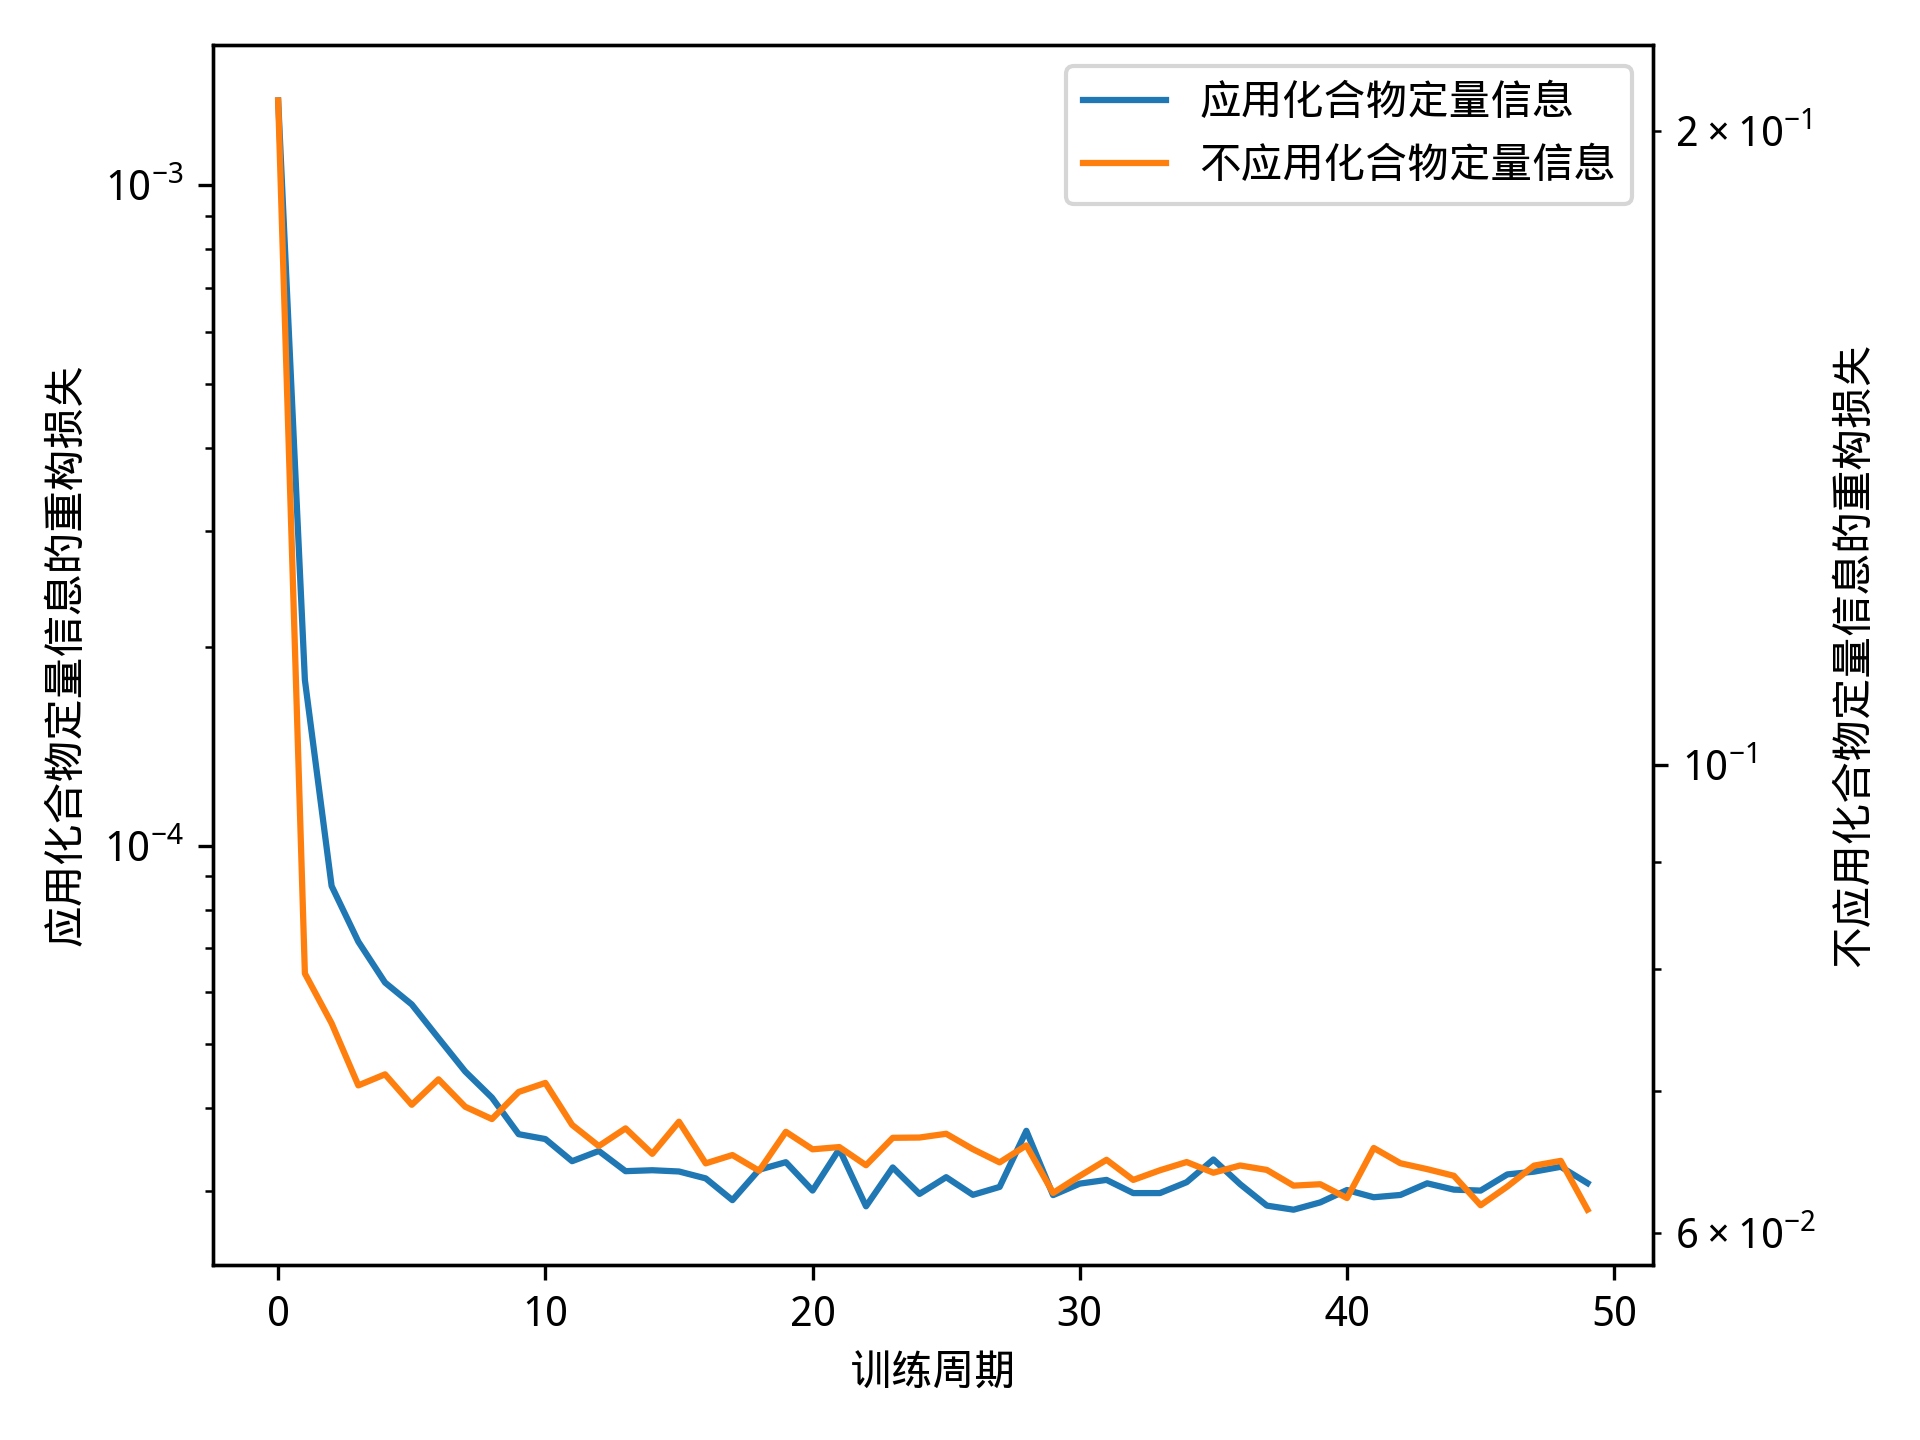
\includegraphics[width=\linewidth]{training_curve.png}
  \caption{使用和不使用化合物定量信息的自编码器训练曲线}
  \label{fig:ae_train_curve}
\end{figure}

可以看到,虽然具体的数值无法直接比较,但是使用化合物信息在自编码器上训练将损失降低了将近两个数量级,而不使用时仅下降到原来的三分之一左右,这可能说明两者学习到特征表示的程度有较大的区别,使用化合物信息的自编码器更好地学习到了处方的特征表示。然后,我们在无化合物含量信息的模型上同样使用各种分类器进行预测,得到相应的预测效果。

\begin{table}[H]
  \centering
  \resizebox{\textwidth}{!}{%
    \begin{tabular}{lcccccccccc}
      \toprule
      \multirow{2}{*}{模型} & \multirow{2}{*}{准确率} & \multicolumn{3}{c}{正例} & \multicolumn{3}{c}{负例} & \multicolumn{3}{c}{加权平均}                                           \\
                          &                      & 精确率                    & 召回率                    & F1                       & 精确率  & 召回率  & F1   & 精确率  & 召回率  & F1   \\
      \midrule
      逻辑回归                & 0.432                & 0.41                   & 0.34                   & 0.37                     & 0.45 & 0.52 & 0.48 & 0.43 & 0.43 & 0.43 \\
      支持向量机               & 0.512                & 0.51                   & 0.50                   & 0.50                     & 0.52 & 0.52 & 0.52 & 0.51 & 0.51 & 0.51 \\
      随机森林                & 0.642                & 0.61                   & 0.76                   & 0.68                     & 0.69 & 0.52 & 0.60 & 0.65 & 0.64 & 0.64 \\
      梯度提升                & 0.580                & 0.56                   & 0.72                   & 0.63                     & 0.62 & 0.44 & 0.51 & 0.59 & 0.58 & 0.57 \\
      AdaBoost            & 0.506                & 0.50                   & 0.62                   & 0.56                     & 0.52 & 0.39 & 0.44 & 0.51 & 0.51 & 0.50 \\
      多层感知机               & 0.481                & 0.48                   & 0.57                   & 0.52                     & 0.48 & 0.39 & 0.43 & 0.48 & 0.48 & 0.48 \\
      朴素贝叶斯               & 0.451                & 0.43                   & 0.33                   & 0.37                     & 0.47 & 0.57 & 0.51 & 0.45 & 0.45 & 0.44 \\
      K近邻                 & 0.512                & 0.51                   & 0.62                   & 0.56                     & 0.52 & 0.40 & 0.46 & 0.51 & 0.51 & 0.51 \\
      \bottomrule
    \end{tabular}
  }
  \caption{只应用基因关联的自编码器各分类器性能对比}
  \label{tab:unweighted_performance_comparison}
\end{table}

直接观察两表,可以看出在大部分分类器和评价指标中,使用化合物定量信息的自编码器的性能要优于不使用的情况,随机森林依然是表现最好的分类器,而在这个分类器上,每一项评价指标的数值均有提升,这说明化合物含量信息的引入对于模型的性能有一定的提升作用。对于以下讨论的其他处理下的分类问题,也具有类似的明显分别,不使用化合物信息的模型性能普遍较差,不再展示相关的实验结果。

之前讨论过,一方面处方过大可能导致在训练集和测试集中的随机分类出现不均衡,但另一方面这些较大的基因关联网络又可能提供更多的基因关联信息,故我们也使用自编码器和不同的分类器来决定是否应该去掉这些较大的处方。在这里,我们将训练集和验证集的处方大小均限制在8及以下,得到的结果如下:

\begin{table}[htbp]
  \centering
  \resizebox{\textwidth}{!}{%
    \begin{tabular}{lcccccccccc}
      \toprule
      \multirow{2}{*}{模型} & \multirow{2}{*}{准确率} & \multicolumn{3}{c|}{正例} & \multicolumn{3}{c|}{负例} & \multicolumn{3}{c|}{加权平均}                                           \\
                          &                      & 精确率                     & 召回率                     & F1                        & 精确率  & 召回率  & F1   & 精确率  & 召回率  & F1   \\
      \midrule
      逻辑回归                & 0.529                & 0.57                    & 0.53                    & 0.55                      & 0.49 & 0.53 & 0.51 & 0.53 & 0.53 & 0.53 \\
      支持向量机               & 0.565                & 0.58                    & 0.72                    & 0.64                      & 0.54 & 0.39 & 0.45 & 0.56 & 0.57 & 0.55 \\
      随机森林                & 0.652                & 0.69                    & 0.65                    & 0.67                      & 0.62 & 0.66 & 0.64 & 0.65 & 0.65 & 0.65 \\
      梯度提升                & 0.645                & 0.69                    & 0.61                    & 0.65                      & 0.60 & 0.69 & 0.64 & 0.65 & 0.64 & 0.65 \\
      AdaBoost            & 0.507                & 0.54                    & 0.50                    & 0.52                      & 0.47 & 0.52 & 0.49 & 0.51 & 0.51 & 0.51 \\
      多层感知机               & 0.572                & 0.63                    & 0.49                    & 0.55                      & 0.53 & 0.67 & 0.59 & 0.58 & 0.57 & 0.57 \\
      朴素贝叶斯               & 0.536                & 0.54                    & 0.92                    & 0.68                      & 0.50 & 0.09 & 0.16 & 0.52 & 0.54 & 0.44 \\
      K近邻                 & 0.572                & 0.60                    & 0.59                    & 0.60                      & 0.54 & 0.55 & 0.54 & 0.57 & 0.57 & 0.57 \\
      \bottomrule
    \end{tabular}
  }
  \caption{去除大于等于9种药材的处方后自编码器各分类器性能对比}
  \label{tab:reduced_performance_comparison}
\end{table}

从准确率的角度而言,去除较大的处方后,支持向量机、多层感知机和朴素贝叶斯的性能在数值上有所提升,而其它分类器的性能下降。性能最高的随机森林分类器性能下降。需要注意的是,这还仅为在处方大小为8及以下的情况下的结果,而更大的真实处方还完全没有引入到评测,相应的特征是未学习的。因此,总体而言,尽管去除较大的处方可能有助于数据集的稳定性,但是在实际的预测中,这些处方可能仍然具有重要的信息,去除后会导致模型性能的下降。